% !TEX root = task-3-9-1.tex
% Editable task bank. Append new BankTask blocks at the end of the document.
\documentclass[12pt,a4paper]{article}
\usepackage{physics-textbook}
\usepackage{graphicx,needspace}
\usetikzlibrary{decorations.pathmorphing}
\newif\ifShowSolutions
\ifdefined\TutorEdition
  \ShowSolutionstrue
\else
  \ShowSolutionsfalse % Change to \ShowSolutionstrue to display solutions.
\fi
\newcounter{banktask}
\newsavebox{\BankTaskBox}
\newcommand{\BankTaskContent}[3]{%
  \noindent\textbf{\thebanktask.}\quad #2\par
  \ifShowSolutions
    \Needspace{50mm}% Keep the solution heading with its opening text or diagram.
    #3\par
    \ifdefined\TutorEdition
      \ifcsname TutorSource#1\endcsname
        \nopagebreak\smallskip{\small\csname TutorSource#1\endcsname\par}%
      \fi
    \fi
  \fi
}
\newcommand{\BankTask}[3]{%
  \refstepcounter{banktask}\par\medskip
  \sbox{\BankTaskBox}{\begin{minipage}{\linewidth}%
    \BankTaskContent{#1}{#2}{#3}\end{minipage}}%
  \ifdim\dimexpr\ht\BankTaskBox+\dp\BankTaskBox\relax>\dimexpr\textheight-20mm\relax
    \Needspace{35mm}\BankTaskContent{#1}{#2}{#3}%
  \else
    \Needspace{\dimexpr\ht\BankTaskBox+\dp\BankTaskBox\relax}%
    \noindent\usebox{\BankTaskBox}\par
  \fi
  \medskip
}
\begin{document}
\BookSubsection{3.9.1}{Закон Ома для участка цепи}


% Source sdamgia-5381: https://phys-ege.sdamgia.ru/problem?id=5381
\BankTask{sdamgia-5381}{
Установите соответствие между формулами для вычисления физических величин в схемах постоянного тока и названиями этих величин.\par
В формулах использованы обозначения: $I$ — сила тока; $U$ — напряжение; $R$ — сопротивление резистора.\par

\begin{center}\begin{minipage}[t]{.47\linewidth}\textbf{Формулы}\par\smallskip А) $\frac{ U}{ I }$\par
Б) $\frac{ U ^2 }{ R }$\end{minipage}\hfill\begin{minipage}[t]{.47\linewidth}\textbf{Физические величины}\par\smallskip $1$. Заряд, протекший через резистор\par
$2$. Сила тока через резистор\par
$3$. Мощность тока, выделяющаяся на резисторе\par
$4$. Сопротивление резистора\end{minipage}\end{center}
\par
\begin{center}\small\setlength{\tabcolsep}{3pt}\begin{tabular}{|p{0.45\linewidth}|p{0.45\linewidth}|}\hline
$A$ & Б\\\hline
 & \\\hline
\end{tabular}\end{center}\par
}{
\smallskip\noindent\textbf{Решение}\par
А) По закону Ома $\frac{ U}{ I } =R.$\par
Б) По закону Джоуля — Ленца мощность тока, которая выделяется в проводнике, равна $\frac{ U ^2 }{ R } .$\par
Ответ: $43$.\par
}

% Source sdamgia-3145: https://phys-ege.sdamgia.ru/problem?id=3145
\BankTask{sdamgia-3145}{
К концам длинного однородного проводника приложено напряжение $U$. Провод удлинили вдвое и приложили к нему прежнее напряжение $U$. Как изменили при этом: силу тока в проводнике, сопротивление проводника и выделяющуюся в проводнике тепловую мощность?\par
$1$. Увеличили.\par
$2$. Уменьшили.\par
$3$. Не изменили.\par
\begin{center}\small\setlength{\tabcolsep}{3pt}\begin{tabular}{|p{0.3\linewidth}|p{0.3\linewidth}|p{0.3\linewidth}|}\hline
Сила тока 
в проводнике & Сопротивление 
проводника & Мощность 
выделяющегося 
в проводнике тепла\\\hline
 &  & \\\hline
\end{tabular}\end{center}\par
}{
\smallskip\noindent\textbf{Решение}\par
Сопротивление длинного однородного проводника пропорционально его длине: $R= \frac{ \rho l}{ S } .$ Следовательно, если удлинить его вдвое, сопротивление увеличится. Согласно закону Ома, сила тока в проводнике связана с его сопротивлением и приложенным к нему напряжением соотношением $I= \frac{ U}{ R } .$ Таким образом, при удлинении проводника и неизменном напряжении сила тока в проводнике уменьшается. Наконец, мощность тока пропорциональна квадрату напряжения и обратно пропорциональна сопротивлению $P= \frac{ U ^2 }{ R } .$ Отсюда получаем, что мощность тока уменьшится в результате удлинения проводника.\par
Ответ: $212$.\par
}

% Source sdamgia-1407: https://phys-ege.sdamgia.ru/problem?id=1407
\BankTask{sdamgia-1407}{
На рисунке изображен график зависимости силы тока в проводнике от напряжения между его концами.\par
Чему равно сопротивление проводника? (В кОм.)\par

\begin{center}\begin{tikzpicture}[book diagram,>=stealth]
\draw[task grid,step=.5](0,0)grid(3,2.5);\draw[task axis](0,0)--(3.3,0)node[right]{$U,\,\text{В}$};\draw[task axis](0,0)--(0,2.8)node[left]{$I,\,\text{мА}$};\node[below left]at(0,0){$0$};\foreach\x in{2,4,6,8}\node[below]at(\x/4,0){$\x$};\foreach\y in{2,4,6}\node[left]at(0,\y/4){$\y$};\draw[task curve](0,0)--(2.4,.6);
\end{tikzpicture}\end{center}
\par
}{
\smallskip\noindent\textbf{Решение}\par
Согласно закону Ома, сила тока, сопротивление проводника и напряжение между его концами связаны соотношением $U=IR.$ Используя график, находим сопротивление проводника $R= \frac{ U}{ I } = \frac{ 8\,\text{В}}{ 2\,\text{мА} } =4\,\text{кОм}.$\par
Ответ: $4$.\par
}

% Source sdamgia-2519: https://phys-ege.sdamgia.ru/problem?id=2519
\BankTask{sdamgia-2519}{
Исследовалась зависимость напряжения на участке цепи от сопротивления этого участка. Результаты измерений представлены в таблице. Погрешности измерений величин $U$ и $R$ равнялись соответственно $0{,}2 \,\text{В}$ и $0{,}5 \,\text{Ом}$. Чему равна сила тока на этом участке цепи? (В амперах с точностью до $0{,}5 \,\text{А}$.)\par
\begin{center}\small\setlength{\tabcolsep}{3pt}\begin{tabular}{|p{0.129\linewidth}|p{0.129\linewidth}|p{0.129\linewidth}|p{0.129\linewidth}|p{0.129\linewidth}|p{0.129\linewidth}|p{0.129\linewidth}|}\hline
$R,\,\text{Ом}$ & $0$ & $1$ & $2$ & $3$ & $4$ & $5$\\\hline
$U,\,\text{В}$ & $0$ & $1{,}8$ & $4{,}2$ & $5{,}8$ & $8{,}4$ & $11{,}6$\\\hline
\end{tabular}\end{center}\par
}{
\smallskip\noindent\textbf{Решение}\par
Рассчитаем для каждого измерения силу тока $( I= \frac{ U}{ R } )$ и усредним получившиеся значения.\par
\begin{center}\small\setlength{\tabcolsep}{3pt}\begin{tabular}{|p{0.129\linewidth}|p{0.129\linewidth}|p{0.129\linewidth}|p{0.129\linewidth}|p{0.129\linewidth}|p{0.129\linewidth}|p{0.129\linewidth}|}\hline
$R,\,\text{Ом}$ & $0$ & $1$ & $2$ & $3$ & $4$ & $5$\\\hline
$U,\,\text{В}$ & $0$ & $1{,}8$ & $4{,}2$ & $5{,}8$ & $8{,}4$ & $11{,}6$\\\hline
$I,\,\text{А}$ & — & $1{,}8$ & $2{,}1$ & $1{,}9$ & $2{,}1$ & $2{,}3$\\\hline
\end{tabular}\end{center}\par
Среднее значение равно\par
\[\frac{ 1{,}8 + 2{,}1 + 1{,}9 + 2{,}1 + 2{,}3}{ 5 } \approx 2{,}0\,\text{А}.\]
Ответ: $2{,}0$.\par
}

% Source sdamgia-1408: https://phys-ege.sdamgia.ru/problem?id=1408
\BankTask{sdamgia-1408}{
На фотографии — электрическая цепь. Показания вольтметра даны в вольтах. Чему будут равны показания вольтметра, если его подключить параллельно резистору $2 \,\text{Ом}$? (В вольтах.) Вольтметр считать идеальным.\par

\begin{center}\begin{tikzpicture}[book diagram,>=stealth]
\draw(0,0)--(0,2)--(.6,2)(1.2,2)--(2,2)(3,2)--(3.5,2)(4.5,2)--(5,2)(6,2)--(6.5,2)--(6.5,0)--(4.5,0)--(4.5,.8)--(3.7,.8)--(3.7,.15);\draw(3.2,0)--(1.2,0)(1,0)--(0,0);\draw[very thick](1,-.35)--(1,.35)(1.2,-.2)--(1.2,.2);\foreach\x/\s in{2/1,3.5/2,5/3}{\draw[fill=gray!10](\x,1.85)rectangle(\x+1,2.15);\node[above]at(\x+.5,2.15){$\s\,\text{Ом}$};}\draw(2,2)--(2,3)--(2.25,3)(2.75,3)--(3,3)--(3,2);\draw(2.5,3)circle(.25)node{$V$};\node[above]at(2.5,3.4){$0{,}6\,\text{В}$};\draw[fill=gray!10](3.2,-.15)rectangle(4.2,.15);\draw[->](3.7,.8)--(3.7,.15);\node[below]at(3.7,-.15){$0\text{--}6\,\text{Ом}$};\fill(.6,2)circle(2pt)(1.2,2)circle(2pt);\draw(.6,2)--(1.35,2.08);
\end{tikzpicture}\end{center}
\par
}{
\smallskip\noindent\textbf{Решение}\par
Согласно закону Ома, сила тока, сопротивление проводника и напряжение между его концами связаны соотношением $U=IR.$ Поскольку резистор $1 \,\text{Ом}$ и резистор $2 \,\text{Ом}$ подключены последовательно, сила тока, текущего через них, совпадает. Следовательно, идеальный вольтметр, подключенный параллельно к резистору $2 \,\text{Ом}$, покажет напряжение:\par
\[U_{2}= \frac{ U_{1}}{ R_{1} } R_{2}= \frac{ 0{,}6\,\text{В}}{ 1\,\text{Ом} } \cdot 2\,\text{Ом}=1{,}2\,\text{В}.\]
Ответ: $1{,}2$.\par
}

% Source sdamgia-3332: https://phys-ege.sdamgia.ru/problem?id=3332
\BankTask{sdamgia-3332}{
Два резистора включены в электрическую цепь параллельно, как показано на рисунке. Значения силы тока в резисторах $I_{1}=0{,}8\,\text{А},$ $I_{2}=0{,}2\,\text{А}.$ Чему равно отношение сопротивлений резисторов $\frac{ R_{1}}{ R_{2} }$?\par

\begin{center}\begin{tikzpicture}[book diagram,>=stealth]
\draw(-.7,0)--(0,0)--(1, .6)--(1.6,.6)(2.6,.6)--(3.2,.6)--(4.2,0)--(4.9,0);\draw(0,0)--(1,-.6)--(1.6,-.6)(2.6,-.6)--(3.2,-.6)--(4.2,0);\foreach\y/\s in{.6/1,-.6/2}{\draw[fill=gray!10](1.6,\y-.15)rectangle(2.6,\y+.15);\node[above]at(2.1,\y+.2){$R_\s$};}\draw[->](3.85,.5)--(2.85,.95)node[midway,above]{$I_1$};\draw[->](3.85,-.5)--(2.85,-.95)node[midway,below]{$I_2$};
\end{tikzpicture}\end{center}
\par
}{
\smallskip\noindent\textbf{Решение}\par
При параллельном соединении напряжения на резисторах совпадают. Согласно закону Ома для участка цепи: $U=IR.$ Следовательно:\par
\[I_{1}R_{1}=I_{2}R_{2} \Longleftrightarrow \frac{ R_{1}}{ R_{2} } = \frac{ I_{2}}{ I_{1} } = \frac{ 0{,}2\,\text{А}}{ 0{,}8\,\text{А} } =0{,}25.\]
Ответ: $0{,}25$.\par
}

% Source sdamgia-24955: https://phys-ege.sdamgia.ru/problem?id=24955
\BankTask{sdamgia-24955}{
На графике показана зависимость силы тока $I$, текущего в цилиндрическом медном проводнике с площадью поперечного сечения $3{,}4 \,\text{мм}^{2}$, от приложенного к его концам напряжения $U$. Удельное сопротивление меди $0{,}017 \,\text{Ом} \cdot \,\text{мм}^{2}/\,\text{м}$.\par
Чему равна длина этого проводника? (В метрах.)\par

\begin{center}\begin{tikzpicture}[book diagram,>=stealth]
\draw[task grid,xstep=1,ystep=.5](0,0)grid(3,3);\draw[task axis](0,0)--(3.4,0)node[right]{$U,\,\text{В}$};\draw[task axis](0,0)--(0,3.4)node[above]{$I,\,\text{А}$};\node[below left]at(0,0){$0$};\foreach\x/\s in{1/.5,2/1.0}{\node[below]at(\x,0){$\s$};}\foreach\y in{1,2}\node[left]at(0,\y){$\y$};\draw[task curve](.8,.8)--(2.75,2.75);
\end{tikzpicture}\end{center}
\par
}{
\smallskip\noindent\textbf{Решение}\par
Сопротивление проводника равно $R= \frac{ U}{ I } ,$ $R= \frac{ \rho l}{ S } .$ Следовательно:\par
\[l= \frac{ US}{ \rho I } = \frac{ 1 \cdot 3{,}4}{ 2 \cdot 0{,}017 } =100\,\text{м}.\]
Ответ: $100$.\par
}

% Source sdamgia-1916: https://phys-ege.sdamgia.ru/problem?id=1916
\BankTask{sdamgia-1916}{
В схеме, изображенной на рисунке, ЭДС источника тока равна $6 \,\text{В}$, его внутреннее сопротивление пренебрежимо мало, а сопротивления резисторов $R_{1}=R_{2}=2 \,\text{Ом}.$ Какое напряжение показывает идеальный вольтметр?\par

\begin{center}\begin{tikzpicture}[book diagram,>=stealth]
\draw(0,0)--(0,1)(0,1.2)--(0,2.5)--(3,2.5)--(3,1.55)(3,.95)--(3,0)--(1.8,0)(1,0)--(0,0);\draw[very thick](-.4,1.2)--(.4,1.2)(-.2,1)--(.2,1);\node[left]at(-.4,1.3){$\mathcal E$};\draw[fill=gray!10](1,-.15)rectangle(1.8,.15);\node[above]at(1.4,.15){$R_1$};\draw[fill=gray!10](2.85,.95)rectangle(3.15,1.55);\node[left]at(2.85,1.25){$R_2$};\draw(3,2)--(4,2)--(4,1.5)(4,1)--(4,.5)--(3,.5);\draw(4,1.25)circle(.25)node{$V$};
\end{tikzpicture}\end{center}
\par
}{
\smallskip\noindent\textbf{Решение}\par
Поскольку внутренним сопротивлением источника можно пренебречь, а вольтметр идеальный, закон Ома приобретает вид $I= \frac{ \mathcal E }{ R } ,$ причем, при последовательно соединении проводников $R=R_{1} + R_{2}.$ Тогда получаем равенство:\par
\[\mathcal E =I ( R_{1} + R_{2} ) .\]
Следовательно, идеальный вольтметр показывает напряжение на втором резисторе, которое по закону Ома для участка цепи равно $U_{2}=I_{2}R_{2}.$ При этом при последовательном соединении $I_{2}=I.$ Таким образом, получаем:\par
\[U_2=\frac{\mathcal E R_2}{R_1+R_2}=\frac{6\,\text{В}\cdot2\,\text{Ом}}{2\,\text{Ом}+2\,\text{Ом}}=3\,\text{В}.\]
Ответ: $3 \,\text{В}$.\par
}

% Source sdamgia-11948: https://phys-ege.sdamgia.ru/problem?id=11948
\BankTask{sdamgia-11948}{
Медный прямой проводник расположен в однородном магнитном поле, модуль вектора магнитной индукции которого равен $20 \,\text{мТл}$. Силовые линии магнитного поля направлены перпендикулярно проводнику. К концам проводника приложено напряжение $3{,}4 \,\text{В}$. Определите площадь поперечного сечения проводника, если сила Ампера, действующая на него, равна $6 \,\text{Н}$. Удельное сопротивление меди равно $1{,}7 \cdot 10^{-8} \,\text{Ом}\cdot\text{м}$.\par
}{
\smallskip\noindent\textbf{Решение}\par
Сила тока в проводнике по закону Ома равна $I = \frac{ U}{ R } .$ Сопротивление проводника равно: $R = \rho \frac{ l}{ S } .$\par
Сила Ампера, действующая на проводник с током, расположенный перпендикулярно линия магнитного поля, вычисляется по формуле: $F_{A} = IBl .$ Тогда получаем:\par
\[F_{A} = IBl = \frac{ U}{ R } Bl = \frac{ US}{ \rho l } Bl = \frac{ USB}{ \rho } .\]
Откуда площадь поперечного сечения проводника равна:\par
\[S = \frac{ F_{\text{А}}\rho}{ UB } = \frac{ 6\,\text{Н} \cdot 1{,}7 \cdot 10 ^{ - 8 } \,\text{Ом} \cdot \,\text{м}}{ 3{,}4\,\text{В} \cdot 20 \cdot 10 ^{ - 3 } \,\text{Тл} } = 1{,}5 \cdot 10 ^{ - 6 } \,\text{м} ^2 = 1{,}5\,\text{мм} ^2 .\]
Ответ: $1{,}5 \,\text{мм}^{2}$.\par
}

% Source sdamgia-25421: https://phys-ege.sdamgia.ru/problem?id=25421
\BankTask{sdamgia-25421}{
На рисунке изображена зависимость силы тока в лампе накаливания от приложенного к ней напряжения. Найдите общее напряжение на источнике тока для цепи, содержащей включенные последовательно резистор и лампу, если сила тока в цепи равна $0{,}4 \,\text{А}$, а мощность, выделяющаяся на резисторе, равна $32 \,\text{Вт}$.\par

\begin{center}\begin{tikzpicture}[book diagram,>=stealth]
\draw[task grid,step=.2](0,0)grid(4.2,2);\draw[task axis](0,0)--(4.5,0)node[right]{$U,\,\text{В}$};\draw[task axis](0,0)--(0,2.2)node[left]{$I,\,\text{А}$};\node[below left]at(0,0){$0$};\foreach\x in{40,80,120,160}\node[below]at(\x/50,0){$\x$};\foreach\y/\s in{.4/{0{,}1},.8/{0{,}2},1.2/{0{,}3},1.6/{0{,}4}}\node[left]at(0,\y){$\s$};\draw[task curve](0,0)..controls(.25,.65)and(1.5,1.26)..(2.8,1.6)..controls(3.2,1.7046153846)and(3.6,1.85)..(4,1.92);
\end{tikzpicture}\end{center}
\par
}{
\smallskip\noindent\textbf{Решение}\par
При последовательном соединении лампы и резистора сила тока через них будет одинаковой. Тогда по графику можем найти напряжение на лампе при силе тока $0{,}4 \,\text{А}$, оно равно $U_{1}\approx140\,\text{В}.$ Зная мощность тока и силу тока через резистор, найдем напряжение на нем $P_{2}=IU_{2},$ откуда $U_{2}= \frac{ P_{2}}{ I } = \frac{ 32}{ 0{,}4 } =80\,\text{В}.$ Общее напряжение при последовательном соединении равно напряжению на источнике:\par
\[U=U_{1} + U_{2}=140 + 80=220\,\text{В}.\]
Ответ: $220 \,\text{В}$.\par
}


% Source 648474: https://ege.fipi.ru/bank/questions.php?search=1&proj=BA1F39653304A5B041B656915DC36B38&qid=648474
\BankTask{648474}{
На рисунке показан график зависимости силы тока в проводнике от напряжения между его концами. Чему равно сопротивление проводника?
\begin{center}
\begin{tikzpicture}[x=0.48cm,y=0.48cm,>=stealth]
\draw[->] (0,0)--(12,0) node[right] {$U,\,\text{В}$};
\draw[->] (0,0)--(0,7.8) node[left] {$I,\,\text{А}$};
\foreach \x in {2,4,6,8,10} {
\foreach \a/\b in {0/0.55,1.85/3.15,4.5/5.8,5.98/6}\draw (\x,\a)--(\x,\b);
\draw (\x,0.12)--(\x,-0.12) node[below] {$\x$};
}
\foreach \y in {2,4,6} {
\foreach \a/\b in {0.22/1.48,2.84/4.10,5.46/6.72,8.09/9.35,9.9/10}\draw (\a,\y)--(\b,\y);
\draw (0.12,\y)--(-0.12,\y) node[left] {$\y$};
}
\node[below left] at (0,0) {$0$};
\draw[very thick] (0,0)--(10,3.3333);
\end{tikzpicture}
\end{center} (в $\text{Ом}$).
}{
\smallskip\noindent\textbf{Решение от GPT}\par
По графику при $U=6\,\text{В}$ сила тока $I=2\,\text{А}$. По закону Ома
\[
R=\frac{U}{I}=\frac{6}{2}=3\,\text{Ом}.
\]
Ответ: $3\,\text{Ом}$.
}

% Source 45F97D: https://ege.fipi.ru/bank/questions.php?search=1&proj=BA1F39653304A5B041B656915DC36B38&qid=45F97D
\BankTask{45F97D}{
На фотографии изображена электрическая цепь. Показания вольтметра даны в вольтах, амперметра — в амперах.
\par\begin{center}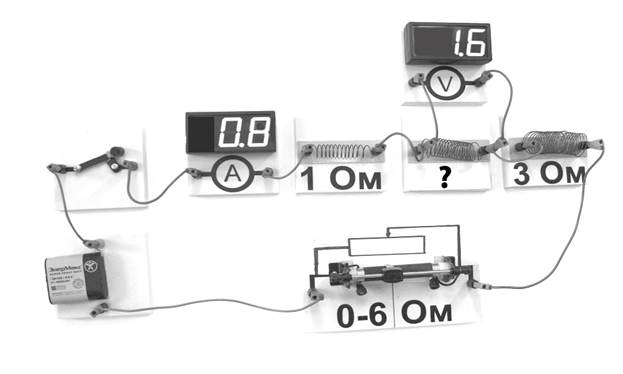
\includegraphics[width=.9\linewidth,height=.48\textheight,keepaspectratio]{_run/photos/11844cc09b6f9596afe3dd1ce24746ab1447feecb4b56a469c4f32a1860fabe4.png}\end{center}\par
Чему равно сопротивление неизвестного резистора (в $\text{Ом}$)? Вольтметр и амперметр считать идеальными.
}{
\smallskip\noindent\textbf{Решение от GPT}\par
По фотографии $I=0{,}8\,\text{А}$, $U=1{,}6\,\text{В}$. По закону Ома
\[
R=\frac{U}{I}=\frac{1{,}6}{0{,}8}=2\,\text{Ом}.
\]
}

% Source 9397C7: https://ege.fipi.ru/bank/questions.php?search=1&proj=BA1F39653304A5B041B656915DC36B38&qid=9397C7
\BankTask{9397C7}{
На фотографии изображена электрическая цепь. Показания вольтметра даны в вольтах.
\par\begin{center}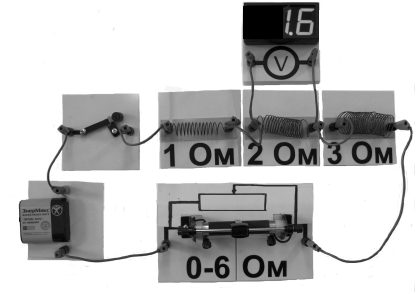
\includegraphics[width=.9\linewidth,height=.48\textheight,keepaspectratio]{_run/photos/389e5d4777aabc394c4661c2152661a8d428c2674ff93ab9ac03afcbdf49c8ea.png}\end{center}\par
Какое напряжение (в $\text{В}$) будет показывать вольтметр, если его подсоединить к резистору сопротивлением $3\,\text{Ом}$? Вольтметр считать идеальным.
}{
\smallskip\noindent\textbf{Решение от GPT}\par
На резисторе $2\,\text{Ом}$ вольтметр показывает $1{,}6\,\text{В}$. Ток в последовательно соединённых резисторах одинаков:
\[
I=\frac{1{,}6}{2}=0{,}8\,\text{А},\qquad U_3=I R_3=0{,}8\cdot3=2{,}4\,\text{В}.
\]
}

% Source 433A84: https://ege.fipi.ru/bank/questions.php?search=1&proj=BA1F39653304A5B041B656915DC36B38&qid=433A84
\BankTask{433A84}{
Электрическая цепь, схема которой изображена на рисунке, подключена к аккумулятору. Напряжение между полюсами аккумулятора равно \(U_0\), а показания идеальных амперметра и вольтметра равны соответственно \(I\) и \(U\).

Установите соответствие между физическими величинами и формулами, по которым их можно рассчитать. Внутренним сопротивлением аккумулятора пренебречь.

\TaskMatchingColumns[0.59\linewidth]{Физические величины}{
А) мощность, потребляемая лампочкой\par
Б) сопротивление лампочки
}{Формулы}{
1) \(\dfrac{U}{I}\)\par
2) \(\dfrac{U_0-U}{I}\)\par
3) \((U_0-U)I\)\par
4) \(UI\)
}

\begin{center}
\begin{tabular}{|c|c|}
\hline
А & Б \\
\hline
\phantom{3} & \phantom{2} \\
\hline
\end{tabular}
\end{center}

\begin{center}
\begin{tikzpicture}[book diagram, x=1cm, y=1cm, line width=0.8pt]
\draw (1.15,1.5) -- (0,1.5) -- (0,1.05);
\draw (0,0.45) -- (0,0) -- (0.5,0);
\draw (0,0.75) circle (0.3);
\node at (0,0.75) {\(\mathrm{A}\)};
\draw (0.8,0) circle (0.3);
\draw (0.59,-0.21) -- (1.01,0.21);
\draw (0.59,0.21) -- (1.01,-0.21);
\draw (1.1,0) -- (1.5,0) -- (2,0);
\draw (2,-0.15) rectangle (2.6,0.15);
\draw (2.6,0) -- (3.05,0) -- (3.05,1.5) -- (1.8,1.5);
\draw (1.5,0) -- (1.5,0.9) -- (1.95,0.9);
\draw (2.25,0.9) circle (0.3);
\node at (2.25,0.9) {\(\mathrm{V}\)};
\draw (2.55,0.9) -- (3.05,0.9);
\fill (1.5,0) circle (0.045);
\fill (3.05,0.9) circle (0.045);
\draw[fill=white] (1.15,1.5) circle (0.06);
\draw[fill=white] (1.8,1.5) circle (0.06);
\node at (1.475,1.88) {\(U_0\)};
\end{tikzpicture}
\end{center}
}{
\smallskip\noindent\textbf{Решение от GPT}\par
Идеальный вольтметр измеряет напряжение на резисторе и не пропускает ток, поэтому через лампочку течёт ток \(I\), а напряжение на ней равно \(U_0-U\). Мощность лампочки \(P=(U_0-U)I\) соответствует формуле 3, её сопротивление \(R=\dfrac{U_0-U}{I}\) — формуле 2. Формулы 1 и 4 определяют соответственно сопротивление и мощность резистора. Ответ: \(32\).
}

% Source BD62B3: https://ege.fipi.ru/bank/questions.php?search=1&proj=BA1F39653304A5B041B656915DC36B38&qid=BD62B3
\BankTask{BD62B3}{
Установите соответствие между формулами для расчёта физических величин в цепях постоянного тока и названиями этих величин. В формулах использованы обозначения: \(R\) — сопротивление резистора; \(P\) — мощность тока в резисторе; \(U\) — напряжение на резисторе.

\TaskMatchingColumns[.35\linewidth]{Формулы}{
А) \(\dfrac{U}{R}\)\par
Б) \(\dfrac{U^2}{P}\)
}{Физические величины}{
1) мощность тока в резисторе\par
2) сопротивление резистора\par
3) сила тока\par
4) количество теплоты, выделяющееся в резисторе
}

\begin{center}
\begin{tabular}{|c|c|}
\hline
А & Б \\
\hline
\phantom{3} & \phantom{2} \\
\hline
\end{tabular}
\end{center}
}{
\smallskip\noindent\textbf{Решение от GPT}\par
По закону Ома \(I=\dfrac{U}{R}\), поэтому А соответствует силе тока (3). Из формулы мощности \(P=\dfrac{U^2}{R}\) получаем \(R=\dfrac{U^2}{P}\), поэтому Б соответствует сопротивлению (2). Мощность (1) равна \(UI\), а количество теплоты (4) равно \(Pt\); ни одна из данных формул их не определяет. Ответ: \(32\).
}

% Source 4963: https://phys-ege.sdamgia.ru/problem?id=4963
\BankTask{4963}{
\begin{center}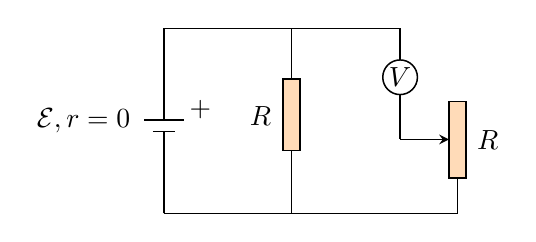
\begin{tikzpicture}[>=stealth,line width=.55pt]\draw(0,0)--(0,1.04) (0,1.19)--(0,2.35)--(3,2.35)--(3,.94) (0,0)--(3.73,0)--(3.73,1.42) (1.62,0)--(1.62,2.35);\draw(-.25,1.19)--(.25,1.19) (-.14,1.04)--(.14,1.04);\draw[->](3,.94)--(3.62,.94);\draw[fill=orange!28](1.51,.8)rectangle(1.73,1.71) (3.62,.45)rectangle(3.84,1.42);\node[left]at(-.3,1.18){$\mathcal E,r=0$};\node[right]at(.2,1.32){$+$};\node[left]at(1.49,1.24){$R$};\node[right]at(3.85,.93){$R$};\draw[fill=white](3,1.73)circle(.22)node{$V$};\end{tikzpicture}\end{center}В схеме на рисунке сопротивление резистора и полное сопротивление реостата равны R, ЭДС батарейки равна Е, ее внутреннее сопротивление ничтожно ($r = 0$). Как ведут себя (увеличиваются, уменьшаются, остаются постоянными) показания идеального вольтметра при перемещении движка реостата из крайнего верхнего в крайнее нижнее положение? Ответ поясните, указав, какие физические закономерности Вы использовали для объяснения.
}{
\smallskip\noindent\textbf{Решение}\par
Вольтметр подключают параллельно к тому участку, на котором нужно измерить напряжение. При этом, естественно, часть тока в цепи начинает течь через сам вольтметр. Тем самым вольтметр вносит возмущение в цепь и показывает напряжение, которое отличается от реального (когда вольтметра нет). Идеальным вольтметром называют прибор, который данной проблемой не страдает. То есть он имеет бесконечное собственное сопротивление. Действительно, рассмотрим положение ползунка реостата, когда он полностью выключен. При параллельном соединении напряжения совпадают:

\[I_RR=U_V=I_VR_V \Longleftrightarrow I_V= \frac{I_RR}{R_V} =0\]

При перемещении ползунка реостата к бесконечному сопротивлению вольтметра прибавляется конечное сопротивление реостата, при этом вольтметр не перестает быть идеальным, ток через него, а значит, и через реостат не течет. Полное сопротивление цепи не изменяется, а значит, полный ток в цепи также остается неизменным $( R_{\,\text{н}} = \frac{R ( R_V + R_{\,\text{р}} )}{R + R_V + R_{\,\text{р}}} =R ,$ по закону Ома для полной цепи $I= \frac{E}{R_{\,\text{н}}} ) .$) Следовательно, на сопротивлении падает одинаковое напряжение при любом положении ползунка ($U=IR$), то есть показания вольтметра не изменяются.
}

\end{document}
